\documentclass[11pt,a4paper]{report}
\usepackage[tmargin=1cm,rmargin=1in,lmargin=1in,margin=0.25in,bmargin=1cm,footskip=.2in]{geometry}
\title{REAL111-1 24H - Fysikk\\Obligatorisk innlevering 5}
\author{Casper Eide Özdemir-Børretzen}
\date{}
\makeatletter
\newcommand{\institle}{\@title}
\newcommand{\insauthor}{\@author}
\newcommand{\insdate}{\@date}
\makeatother

% % % % % % % % % % % % % % % % % % % % % % % % % % % % % % % % % % % % % % % % 

\usepackage{nicefrac}
\usepackage{mhchem}              % Chemistry symbols
\usepackage{graphicx}            % Images
\usepackage{listings}            % Code
\usepackage{ulem}                % Double underline
\usepackage{amssymb}             %
\usepackage{pdfpages}            % Insert pdf pages
\usepackage{enumitem}            % Lists
\usepackage{titlesec}            %
\usepackage[T1]{fontenc}         %
\usepackage[utf8]{inputenc}      %
\usepackage[fleqn]{amsmath}      %
\usepackage[makeroom]{cancel}    %
\setlength{\parindent}{0pt}
\titlespacing*{\subsection}{0cm}{2cm}{0.5cm}
\lstset{
aboveskip=0cm,
belowskip=0cm,
showstringspaces=false,
columns=flexible,
basicstyle={\scriptsize\ttfamily},
breaklines=true,
breakatwhitespace=true,
tabsize=4,
inputencoding = utf8,  % Input encoding
extendedchars = true,  % Extended ASCII
literate      =        % Support additional characters
{á}{{\'a}}1  {é}{{\'e}}1  {í}{{\'i}}1 {ó}{{\'o}}1  {ú}{{\'u}}1
{Á}{{\'A}}1  {É}{{\'E}}1  {Í}{{\'I}}1 {Ó}{{\'O}}1  {Ú}{{\'U}}1
{à}{{\`a}}1  {è}{{\`e}}1  {ì}{{\`i}}1 {ò}{{\`o}}1  {ù}{{\`u}}1
{À}{{\`A}}1  {È}{{\`E}}1  {Ì}{{\`I}}1 {Ò}{{\`O}}1  {Ù}{{\`U}}1
{ä}{{\"a}}1  {ë}{{\"e}}1  {ï}{{\"i}}1 {ö}{{\"o}}1  {ü}{{\"u}}1
{Ä}{{\"A}}1  {Ë}{{\"E}}1  {Ï}{{\"I}}1 {Ö}{{\"O}}1  {Ü}{{\"U}}1
{â}{{\^a}}1  {ê}{{\^e}}1  {î}{{\^i}}1 {ô}{{\^o}}1  {û}{{\^u}}1
{Â}{{\^A}}1  {Ê}{{\^E}}1  {Î}{{\^I}}1 {Ô}{{\^O}}1  {Û}{{\^U}}1
{œ}{{\oe}}1  {Œ}{{\OE}}1  {æ}{{\ae}}1 {Æ}{{\AE}}1  {ß}{{\ss}}1
{ẞ}{{\SS}}1  {ç}{{\c{c}}}1 {Ç}{{\c{C}}}1 {ø}{{\o}}1  {Ø}{{\O}}1
{å}{{\aa}}1  {Å}{{\AA}}1  {ã}{{\~a}}1  {õ}{{\~o}}1 {Ã}{{\~A}}1
{Õ}{{\~O}}1  {ñ}{{\~n}}1  {Ñ}{{\~N}}1  {¿}{{?`}}1  {¡}{{!`}}1
{„}{\quotedblbase}1 {“}{\textquotedblleft}1 {–}{$-$}1
{°}{{\textdegree}}1 {º}{{\textordmasculine}}1 {ª}{{\textordfeminine}}1
{£}{{\pounds}}1  {©}{{\copyright}}1  {®}{{\textregistered}}1
{«}{{\guillemotleft}}1  {»}{{\guillemotright}}1  {Ð}{{\DH}}1  {ð}{{\dh}}1
{Ý}{{\'Y}}1    {ý}{{\'y}}1    {Þ}{{\TH}}1    {þ}{{\th}}1    {Ă}{{\u{A}}}1
{ă}{{\u{a}}}1  {Ą}{{\k{A}}}1  {ą}{{\k{a}}}1  {Ć}{{\'C}}1    {ć}{{\'c}}1
{Č}{{\v{C}}}1  {č}{{\v{c}}}1  {Ď}{{\v{D}}}1  {ď}{{\v{d}}}1  {Đ}{{\DJ}}1
{đ}{{\dj}}1    {Ė}{{\.{E}}}1  {ė}{{\.{e}}}1  {Ę}{{\k{E}}}1  {ę}{{\k{e}}}1
{Ě}{{\v{E}}}1  {ě}{{\v{e}}}1  {Ğ}{{\u{G}}}1  {ğ}{{\u{g}}}1  {Ĩ}{{\~I}}1
{ĩ}{{\~\i}}1   {Į}{{\k{I}}}1  {į}{{\k{i}}}1  {İ}{{\.{I}}}1  {ı}{{\i}}1
{Ĺ}{{\'L}}1    {ĺ}{{\'l}}1    {Ľ}{{\v{L}}}1  {ľ}{{\v{l}}}1  {Ł}{{\L{}}}1
{ł}{{\l{}}}1   {Ń}{{\'N}}1    {ń}{{\'n}}1    {Ň}{{\v{N}}}1  {ň}{{\v{n}}}1
{Ő}{{\H{O}}}1  {ő}{{\H{o}}}1  {Ŕ}{{\'{R}}}1  {ŕ}{{\'{r}}}1  {Ř}{{\v{R}}}1
{ř}{{\v{r}}}1  {Ś}{{\'S}}1    {ś}{{\'s}}1    {Ş}{{\c{S}}}1  {ş}{{\c{s}}}1
{Š}{{\v{S}}}1  {š}{{\v{s}}}1  {Ť}{{\v{T}}}1  {ť}{{\v{t}}}1  {Ũ}{{\~U}}1
{ũ}{{\~u}}1    {Ū}{{\={U}}}1  {ū}{{\={u}}}1  {Ů}{{\r{U}}}1  {ů}{{\r{u}}}1
{Ű}{{\H{U}}}1  {ű}{{\H{u}}}1  {Ų}{{\k{U}}}1  {ų}{{\k{u}}}1  {Ź}{{\'Z}}1
{ź}{{\'z}}1    {Ż}{{\.Z}}1    {ż}{{\.z}}1    {Ž}{{\v{Z}}}1  {ž}{{\v{z}}}1
}

% % % % % % % % % % % % % % % % % % % % % % % % % % % % % % % % % % % % % % % % 

\newcommand{\m}{\cdot}
\newcommand{\opgd}[1]{\item[#1)]}
\newcommand{\opg}[1]{\subsection*{Oppgave #1}}
\newcommand{\enkelsvaralign}[1]{\makebox[0pt][l]{\uuline{\phantom{$#1$}}}#1}
\newcommand{\svaralign}[2]{\makebox[0pt][l]{\uuline{\phantom{$#1 #2$}}}#1 &#2}

% % % % % % % % % % % % % % % % % % % % % % % % % % % % % % % % % % % % % % % % 

\begin{document}
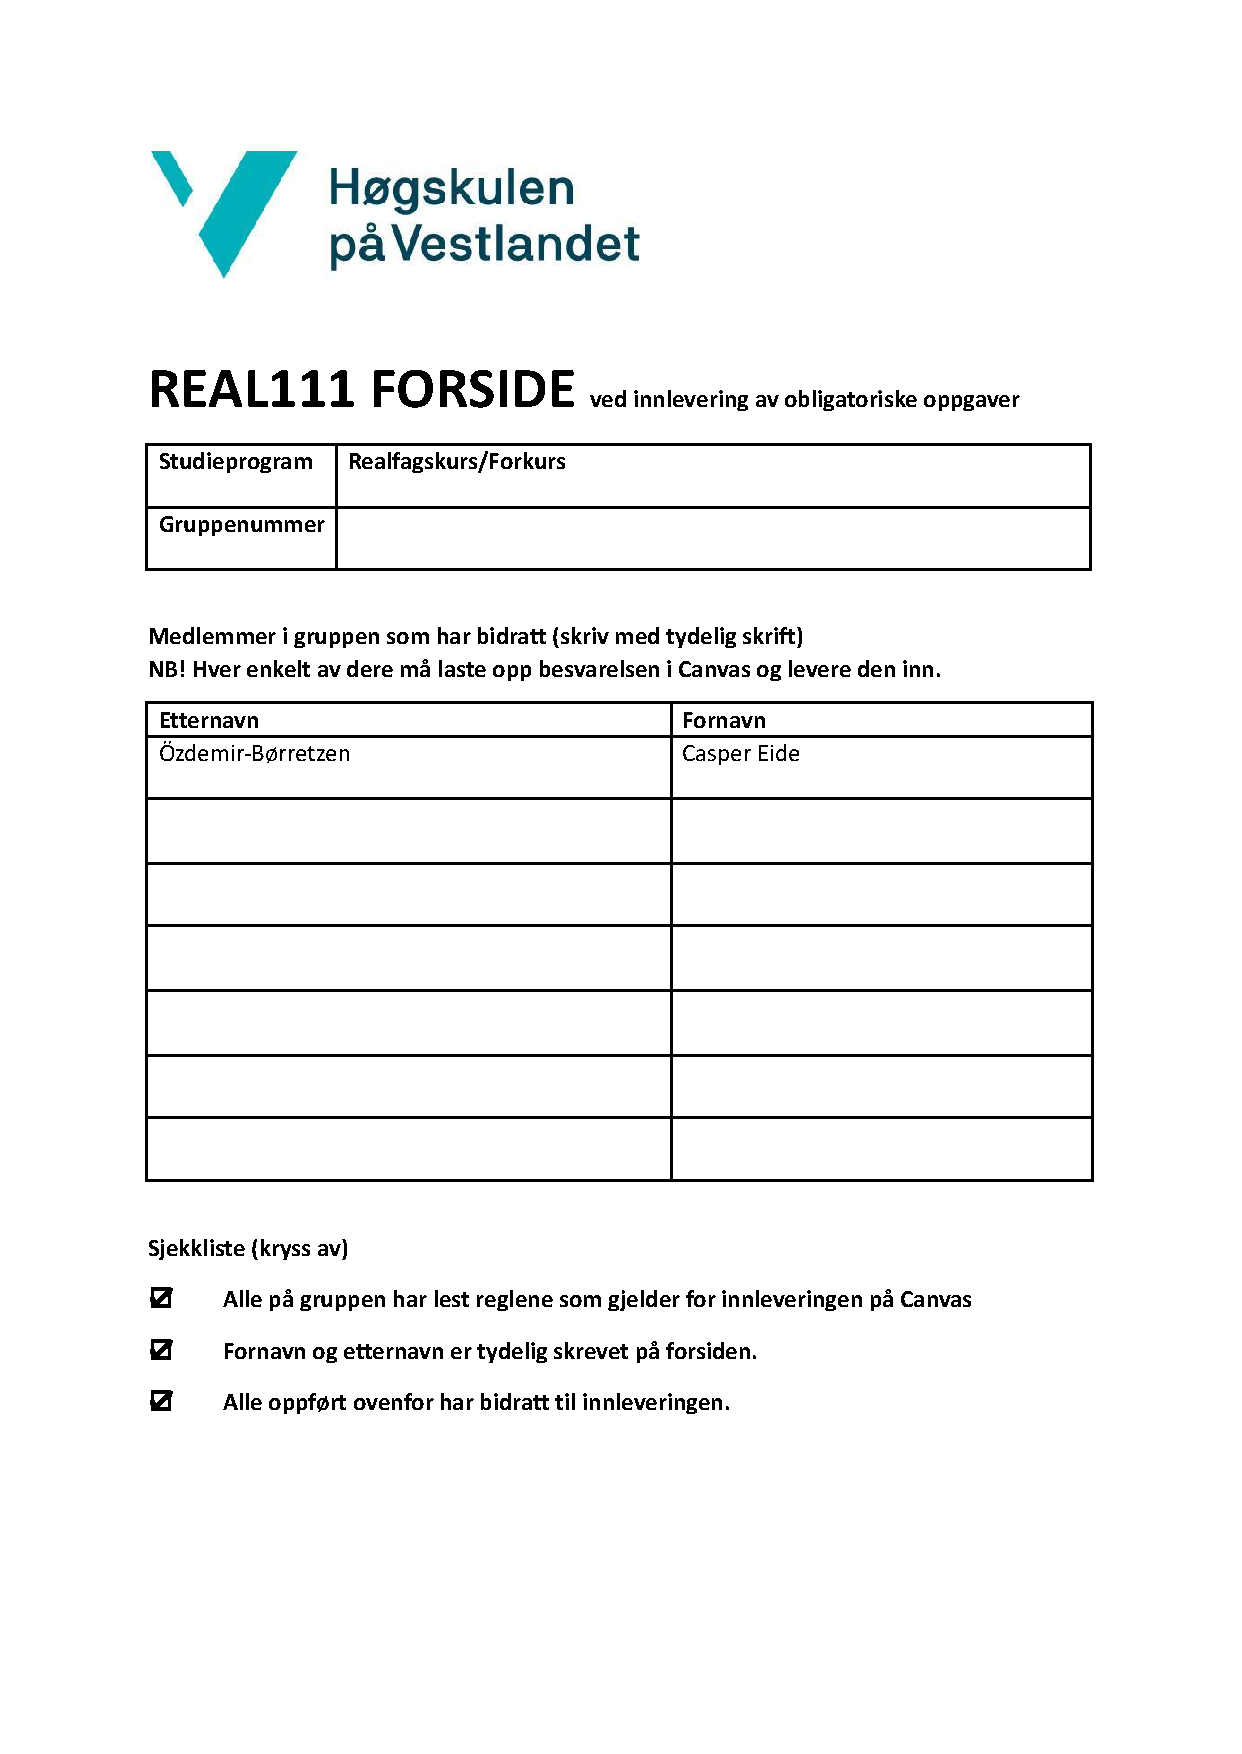
\includepdf[pages={1}]{real111-forside.pdf}

% % % % % % % % % % % % % % % % % % % % % % % % % % % % % % % % % % % % % % % % 

\opg{1}
\begin{enumerate}[leftmargin=*,itemsep=1cm,labelsep=2em,label=\alph*)]
\opgd{a}
\begin{align*}
&v = 340\ m/s\\
&f = 262\ Hz\\
&v = \lambda \cdot f\\
&\lambda = \frac{v}{f} = \frac{340\ m/s}{262\ Hz} = \uuline{1,30\ m}\\
\end{align*}
\opgd{b}
Røntgenstråling:
\begin{align*}
&\lambda = 0,100\ nm\\[0.2cm]
&f = \frac{v}{\lambda} = \frac{c}{\lambda} = \frac{3,00 \cdot 10^8\ m/s}{100 \cdot 10^{-12}\ m} = 3 \cdot 10^{18}\ Hz = \uuline{3,00\ EHz}\\[0.2cm]
&E_f = \frac{hc}{\lambda} = \frac{6,63 \cdot 10^{-34}\ J/s \cdot 3,00 \cdot 10^8\ m/s}{100 \cdot 10^{-12}\ m} = \uuline{1,99 \cdot 10^{-15}\ J}\\[0.2cm]
\end{align*}
Radiobølge:
\begin{align*}
&\lambda = 3,00\ m\\
&f = \frac{v}{\lambda} = \frac{c}{\lambda} = \frac{3,00 \cdot 10^8\ m/s}{3,00\ m} = 10^{8}\ Hz = \uuline{100\ MHz}\\[0.2cm]
&E_f = \frac{hc}{\lambda} = \frac{6,63 \cdot 10^{-34}\ J/s \cdot 3,00 \cdot 10^8\ m/s}{3,00\ m} = \uuline{6,63 \cdot 10^{-23}\ J}\\[0.2cm]
\end{align*}
\end{enumerate}

% % % % % % % % % % % % % % % % % % % % % % % % % % % % % % % % % % % % % % % % 

\newpage
\opg{2}
\begin{enumerate}[leftmargin=*,itemsep=1cm,labelsep=2em,label=\alph*)]
\opgd{a}
I Rutherfords atommodell har atomet en positivt ladd kjerne bestående av protoner og nøytroner, og negativt ladde elektronene som spinner rundt kjernen lik planeter i bane rundt solen. I Bohrs atommodell går elektronene fortsatt i bane rundt kjernen, men elektronene kan stegvis øke avstand fra kjernen hvis atomet blir tilført energi fra et foton. Den laveste energitilstanden kalles grunntilstand, og høyere energitilstander kalles eksiterte energitilstander. Hvis atomets er i en eksitert energitilstand vil det etter en viss tid sende ut energi i form av foton og gå stegvis, enten direkte i ett steg, eller i flere mindre steg, mot grunntilstanden.
\opgd{b}
\begin{align*}
&E_3 = -0,242 \cdot 10^{-18}\ J\\
&E_2 = -0,545 \cdot 10^{-18}\ J\\
&E_1 = -2,18 \cdot 10^{-18}\ J
\end{align*}
Mulige kvantesprang fra $n=3$ til $n=1$ (grunntilstand) er direkte fra $n=3$ til $n=1$ eller i to steg, fra $n=3$ til $n=2$ etterfulgt av $n=2$ til $n=1$
\begin{center}
\line(1,0){450}
\end{center}
Fra $n=3$ til $n=1$:
\begin{align*}
&E_f = E_3 - E_1 = 0,242\ aJ - (-2,18\ aJ) = \uuline{1,938\ aJ}\\[0.2cm]
&f = \frac{E_f}{h} = \frac{1,938 \cdot 10^{-18}\ J}{6,63 \cdot 10^{-34}\ J/s} = 2,923 \cdot 10^{15}\ Hz = \uuline{2,923\ PHz}\\[0.2cm]
&\lambda = \frac{c}{f} = \frac{3,00 \cdot 10^8\ m/s}{2,923 \cdot 10^{15}\ Hz} = 1,026 \cdot 10^{-7}\ m = \uuline{102,6\ nm}
\end{align*}
\begin{center}
\line(1,0){450}
\end{center}
Fra $n=3$ til $n=2$:
\begin{align*}
&E_f = E_3 - E_2 = -0,242\ aJ - (-0,545\ aJ) = \uuline{0,303\ aJ}\\[0.2cm]
&f = \frac{E_f}{h} = \frac{0,303 \cdot 10^{-18}\ J}{6,63 \cdot 10^{-34}\ J/s} = 4,570 \cdot 10^{14}\ Hz = \uuline{457,0\ THz}\\[0.2cm]
&\lambda = \frac{c}{f} = \frac{3,00 \cdot 10^8\ m/s}{4,570 \cdot 10^{14}\ Hz} = 6,565 \cdot 10^{-7} m = \uuline{656,5\ nm}
\end{align*}
\begin{center}
\line(1,0){450}
\end{center}
Fra $n=2$ til $n=1$:
\begin{align*}
&E_f = E_2 - E_1 = -0,545\ aJ - (-2,18\ aJ) = \uuline{1,635\ aJ}\\[0.2cm]
&f = \frac{E_f}{h} = \frac{1,635 \cdot 10^{-18}\ J}{6,63 \cdot 10^{-34}\ J/s} = 2,466 \cdot 10^{15} = \uuline{2,466\ PHz}\\[0.2cm]
&\lambda = \frac{c}{f} = \frac{3,00 \cdot 10^8\ m/s}{2,466 \cdot 10^{15}\ Hz} = 1,217 \cdot 10^{-7}\ m = \uuline{121,7\ nm}
\end{align*}
\end{enumerate}

% % % % % % % % % % % % % % % % % % % % % % % % % % % % % % % % % % % % % % % % 

\newpage
\opg{3}
\begin{enumerate}[leftmargin=*,itemsep=1cm,labelsep=2em,label=\alph*)]
\opgd{a}

{\huge
\begin{align*}
&\ce{^{222}_{86}Rn} \rightarrow \ce{^{4}_{2}He} + \ce{^{A}_{Z}X} + energi
\end{align*}
}%

\begin{align*}
&86 = 2 + Z\\
&Z = 86 - 2 = 84\\
&222 = 4 + A\\
&A = 222 - 4 = 218
\end{align*}

{\huge
\begin{align*}
&\ce{^{A}_{Z}X} = \ce{^{218}_{84}Po}\\[0.5cm]
&\ce{^{222}_{86}Rn} \rightarrow \ce{^{4}_{2}He} + \ce{^{218}_{84}Po} + energi
\end{align*}
}%

\opgd{b}
\begin{align*}
&m_{Rn} = 222\ u\\
&m_{He} = 4,003\ u\\
&m_{Po} = 209\ u\\
&\Delta m = m_{Rn} - m_{He} - m_{Po} = 222\ u - 4,003\ u - 209\ u = 8,997\ u\\
&E_r = \Delta mc^2 = 8,997 \cdot 1,66057 \cdot 10^{-27}\ kg \cdot (3,00 \cdot 10^8\ m/s)^2 = 1,344613346 \cdot 10^{-9}\ J \approx \uuline{1,345 \cdot 10^{-9}\ J}
\end{align*}

\opgd{c}
{\huge
\begin{align*}
&\ce{^{212}_{82}Pb} \rightarrow \ce{^{212}_{83}Bi} + \ce{^{0}_{-1}e} + energi
\end{align*}
}%
\end{enumerate}

% % % % % % % % % % % % % % % % % % % % % % % % % % % % % % % % % % % % % % % % 
\newpage
\opg{4}
\begin{enumerate}[leftmargin=*,itemsep=1cm,labelsep=2em,label=\alph*)]
\opgd{a}
\begin{align*}
&n = \frac{1\ kg \cdot 0,15 \cdot 1,00 \cdot 10^{-12}}{12,01 \cdot 1,66057 \cdot 10^{-27}\ kg} = \uuline{7,521268002 \cdot 10^{12}}
\end{align*}
\opgd{b}
\begin{align*}
&A_0 = 25,0\ Bq\\[0.2cm]
&A = 2,50\ Bq\\[0.2cm]
&t\nicefrac{1}{2} = 6730\ \text{år}\\[0.2cm]
&A = A_0 \cdot (\frac{1}{2})^{\frac{t}{t\nicefrac{1}{2}}}\\[0.2cm]
&\frac{A}{A_0} = (\frac{1}{2})^{\frac{t}{t\nicefrac{1}{2}}}\\[0.2cm]
&\ln(\frac{A}{A_0}) = \frac{t}{t\nicefrac{1}{2}} \cdot \ln(\frac{1}{2})\\[0.2cm]
&t = \frac{\ln(\frac{A}{A_0}) \cdot t\nicefrac{1}{2}}{\ln(\frac{1}{2})}\\[0.2cm]
&t = \frac{\ln(\frac{2,50\ Bq}{25,0\ Bq}) \cdot 5730\ \text{år}}{\ln(\frac{1}{2})}\\[0.2cm]
&t = 19034,64798\ \text{år}\\[0.2cm]
&t \approx \uuline{19\ 035\ \text{år}}
\end{align*}
\end{enumerate}

% % % % % % % % % % % % % % % % % % % % % % % % % % % % % % % % % % % % % % % % 

\newpage
\opg{5}
\begin{enumerate}[leftmargin=*,itemsep=1cm,labelsep=2em,label=\alph*)]
\opgd{a}
\begin{align*}
&A = 4 \pi r^2\\
&T = 9560\ K\\
&r = 2,11 \cdot 10^9\ m\\
&\sigma = 5,67 \cdot 10^{-8}\ \nicefrac{W}{(m^2 K^4)}\\
&P_{ut} = \sigma A T^4 \\
&P_{ut} = 5,67 \cdot 10^{-8} \nicefrac{W}{(m^2 K^4)} \cdot 4 \cdot \pi \cdot (2,11 \cdot 10^9\ m)^2 \cdot (9560\ K)^4 = 2,649655443 \cdot 10^{28}\ W\\
&P_{ut} = \uuline{2650\ YW}
\end{align*}
\opgd{b}
\begin{align*}
%&r = 2,11 \cdot 10^9\ m + 3,00 \cdot 10^8\ m/s \cdot 60\ s \cdot 60 \cdot 24 \cdot 365\\[0.2cm]
&I = \frac{P}{4 \pi r^2} = \frac{2,649655443 \cdot 10^{28}\ W}{4 \pi (2,11 \cdot 10^9\ m + 3,00 \cdot 10^8\ m/s \cdot 60\ s \cdot 60 \cdot 24 \cdot 365)^2}\\[0.2cm]
&I = \uuline{2,355720793 \cdot 10^{-5}\ \nicefrac{W}{m^2}}
\end{align*}
\opgd{c}
\begin{align*}
&\lambda_{topp} = \frac{a}{K}\\[0.2cm]
&K = \frac{a}{\lambda_{topp}}\\[0.2cm]
&\lambda_{topp,1} = 475\ nm\\[0.2cm]
&\lambda_{topp,2} = 575\ nm\\[0.2cm]
&T_1 = \frac{a}{\lambda_{topp,1}} = \frac{2,90 \cdot 10^{-3}\ K \cdot m}{474 \cdot 10^{-9}\ m} = \uuline{6105\ K}\\[0.2cm]
&T_2 = \frac{a}{\lambda_{topp,2}} = \frac{2,90 \cdot 10^{-3}\ K \cdot m}{575 \cdot 10^{-9}\ m} = \uuline{5043\ K}\\[0.2cm]
\end{align*}
\opgd{d}
Figuren visen bølgelengden på stråling fra solen, bølgelengde på strålig fra jorden og hvilke bølgelengder de forskjellige klimagassene kan absorbere. Dette forklarer drivhuseffekten, da stråligen fra solen stort sett går gjennom gassene uten å bli absorbert, mens strålingen fra jorden i mye større grad blir absorbert av gassene og bidrar til å varme opp atmosfæren. Utifra denne figuren kan man også se hvorfor utslipp av $CO_2$ gass bidrar i stor grad til økt drivhuseffekt ettersom $CO_2$ har veldig høy absorpsjon der utstråligstettheten fra jorden er nær det høyeste.
\end{enumerate}

% % % % % % % % % % % % % % % % % % % % % % % % % % % % % % % % % % % % % % % % 

\newpage
\opg{6}
a)\\
\lstinputlisting[language=Python]{6a.py}

\newpage
\opg{6}
b) og c)\\
(som en liten øvelse har jeg gjort flere endringer i programmet, og har lagt inn forklaringer som kommentarer)\\
\lstinputlisting[language=Python]{6bc.py}

\newpage
Grafene som koden produserer:
\begin{center}
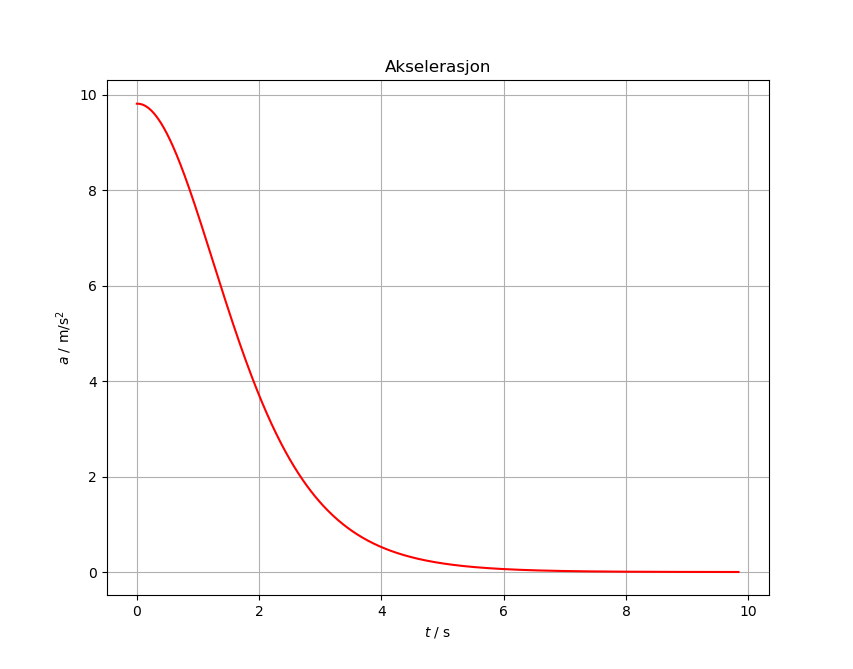
\includegraphics[scale=0.4]{6b1.png}\\\\
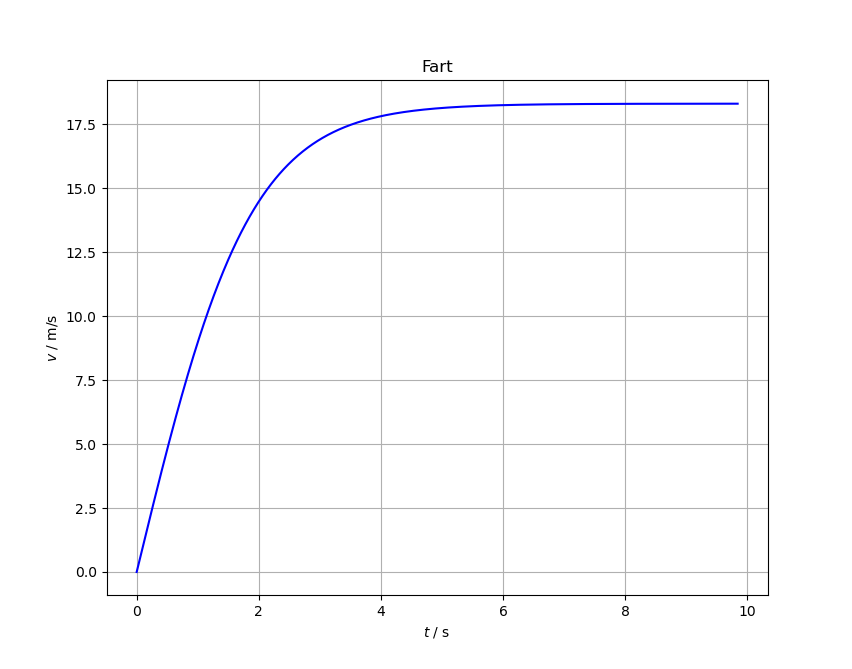
\includegraphics[scale=0.4]{6b2.png}\\\\
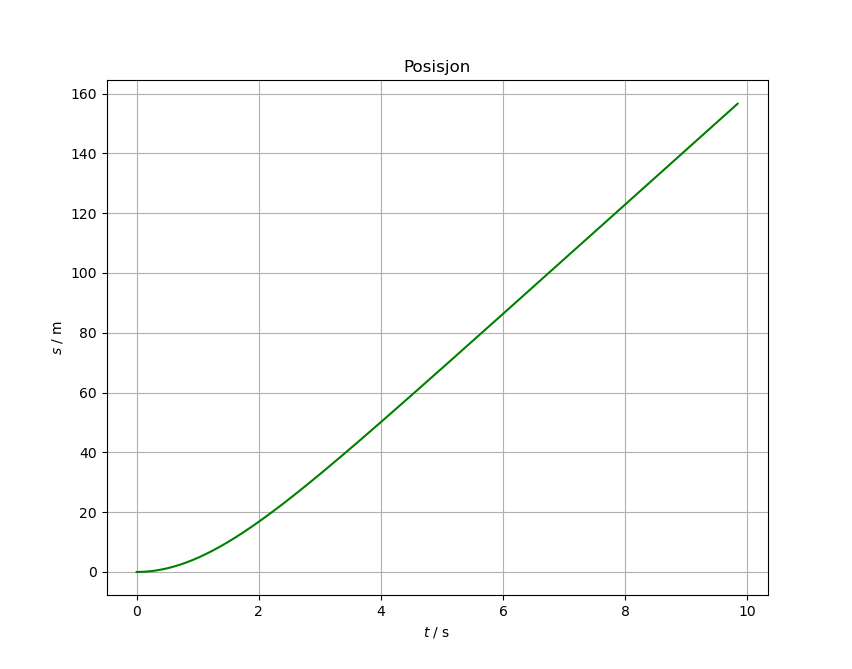
\includegraphics[scale=0.4]{6b3.png}\\\\
\end{center}

\vspace{0.5cm}

d)
Det tar cirka 10 sekunder for å oppnå terminalfart. Farten stemmer med svaret i a.

\newpage
e)\\
\lstinputlisting[language=Python]{6e.py}
\end{enumerate}

\end{document}
